
\renewcommand*\descriptionlabel[1]{\hspace\leftmargin$#1$}
\setcounter{tocdepth}{5}
\setcounter{secnumdepth}{5}
\newcommand{\minus}{\scalebox{0.65}[1.0]{$-$}}

%\section{Notes}

%A 1-gpm
%(0.06 liter/sec) side stream of the primary salt is
%continuously processed to remove
% 233 P a , to recover the
%bred
% 233 U , and to adjust the fissile content. Robertson summary
 
% Robertson does not define thorium feed rate?
 
% Serpent2 continuous reprocessing section cite own presentations at Serpent user group meetings

\section{Batchwise Reprocessing}

SaltProc is used to handle batchwise reprocessing in this work because it provides a batchwise reprocessing scheme which can be customized fairly easily. There are different versions of SaltProc which have slightly different methods in how the depletion data is stored as well as how reprocessing rates are calculated.
%an accurate model of the MSBR, uses Serpent2 for transport and depletion calculations, and because it provides

\subsection{Bulk}

SaltProc version 0.1 is the first full version of SaltProc which was publicly released, and provides all the functionality necessary for modeling the MSBR with batchwise reprocessing. This version uses 3 day steps and does not perform fractional reprocessing at each step, but instead performs reprocessing according to the cycle times, which is termed as the "Bulk" approach to batchwise reprocessing. This is the same approach used by Gehin and Powers for an analysis of the MSBR \cite{gehin_liquid_2016}.

For example, a 30 day cycle time would be implemented as no reprocessing during the first 27 days, then full 100\% removal of the target at the 30 day mark. This works well for reactor processes which are performed batchwise, such as adding uranium to the reactor which can be performed as a batch process. However, for approximating online reprocessing, this approach is not ideal, as it is less able to capture the frequency of the reprocessing.

For the refueling of the reactor, the thorium feed rate was set to maintain the thorium mass in the reactor. The uranium feed rate was set to be equivalent to the protactinium removal rate. This carries an implicit assumption that there is already a backlog of decayed protactinium which has transmuted into uranium which is ready to be pumped back into the core. Both the thorium feed and protactinium to uranium refueling processes occur every 3 days. These refueling rates can be seen in Figures \ref{fig:Th-feed-v1} and \ref{fig:U-feed-v1}, which are recreated from the data from Rykhlevskii \cite{rykhlevskii_advanced_2018}.

% Include figure of U and Th feed rates over time.

\begin{figure}[H]
  \centering
  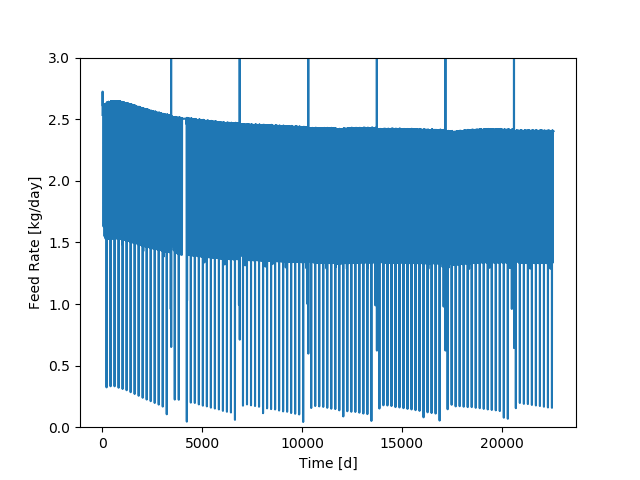
\includegraphics[scale=0.7]{images/Th232rem_massv01.png}
  \caption{Thorium feed rate in the MSBR as a function of time while using bulk batchwise reprocessing \cite{rykhlevskii_advanced_2018}.}
   \label{fig:Th-feed-v1}
\end{figure}

\begin{figure}[H]
  \centering
  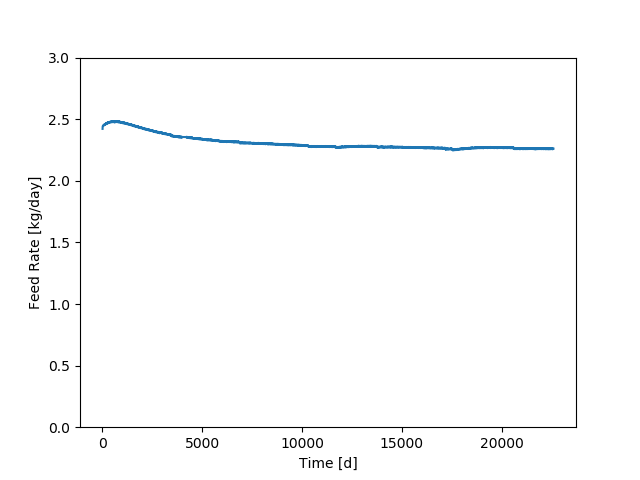
\includegraphics[scale=0.7]{images/Pa233rem_massv01.png}
  \caption{Uranium feed rate in the MSBR as a function of time while using bulk batchwise reprocessing \cite{rykhlevskii_advanced_2018}.}
   \label{fig:U-feed-v1}
\end{figure}

The large jumps in the thorium feed rate are due to the bulk removal of absorbers, leading to spikes in the effective multiplication factor \cite{rykhlevskii_advanced_2018}. The uranium feed rate is smooth because it is based purely on the outflow of protactinium and does not fluctuate as rapidly as the thorium, which is the only external feed in the MSBR system. The average thorium-232 feed rate is 2.38 kg/day, while the average uranium-233 feed rate is 2.31 kg/day. These average values are used as the baseline for feed rates for the other batchwise method and for the continuous methods.

Another difference is that this version makes use of the h5py Python package to handle the hdf5 data files which contain depletion data. Within the hdf5 file, the atom density of each isotope before and after batchwise reprocessing is recorded as well as different reactor parameters such as the neutron multiplication factor.

\subsection{Steady}

SaltProc version 0.3 includes an example MSBR which users can run as soon as SaltProc is installed, though some of the run parameters such as neutrons per generation and run time have to be altered to generate a more valid model. This model also uses 3 day steps, but instead of performing the batch removal only at the cycle time value, this model removes a fraction every 3 days, which is called the "Steady" approach for batchwise reprocessing.

For example, a 30 day cycle time would result in 10\% removal every 3 days. This more accurately models online reprocessing, which is primarily what the MSBR employs in its reprocessing scheme aside from the salt discard.

The reactor refueling is performed slightly differently from v0.1 as well. This version assumes a constant ratio between the uranium refueling and the thorium refueling. The net refueling for each 3 day depletion step is set to maintain the mass of the system. Thus, the average values of 2.38 kg/day and 2.31 kg/day for thorium-232 and uranium-233, respectively, are used to determine the ratio of uranium to thorium which is implemented.

Additionally, this version of SaltProc uses the PyTables Python package for handling the hdf5 data files. The data files are structured similarly to v0.1 of SaltProc, but instead of atom density they use mass, which makes analysis of the files slightly more user friendly.

\subsection{Batch Approaches Summary}

\begin{table}[H]
\renewcommand{\arraystretch}{1.25}
\caption{Batchwise Reprocessing Methods}
\label{tab:batch_methods}
\begin{center}
\begin{tabular}{ | c | c | c | c | c | }
 \hline
        Approach & $\Delta t$ $[s]$ & $T_{cyc}$ $[s]$ & Fractional Removal Rate [s$^{-1}$] & Step Removal\\
 \hline
 \hline
        Bulk & 1 & 20 & - & \, 0/1$^{*}$\\
        Bulk & 10 & 20 & - & \, 0/1$^{*}$ \\
        Bulk & 40 & 20 & - & 1 \\
        Steady & 1 & 20 & 0.05 & 0.05\\
        Steady & 10 & 20 & 0.05 & 0.5\\
        Steady & 40 & 20 & 0.025 & 1\\
 \hline
\end{tabular}
\end{center}
\end{table}
        \begin{center}
\footnotesize{$^{*}$ Bulk removal is 0 until the depletion step is equal to the cycle time, at which point it removes 100\%.}\\
        \end{center}
        
Table \ref{tab:batch_methods} reflects the information shown in Figure \ref{fig:bulk_repr_cnst}. The table shows how the bulk method will only remove 100\% at the cycle time, and otherwise removes nothing. Additionally, the bulk method will remove 100\% as soon as possible if the depletion step size, $\Delta t$, is larger than the cycle time, $T_{cyc}$. 

The table also describes how the steady method fractional removal is constant up until the depletion step size becomes larger than the cycle time, at which point the removal at each step is 100\%, causing the steady method to then be equivalent to the bulk method. However, for shorter times, the steady method allows for a consistent fractional removal rate by adjusting the removal at each step.


\begin{figure}[H]
  \centering
  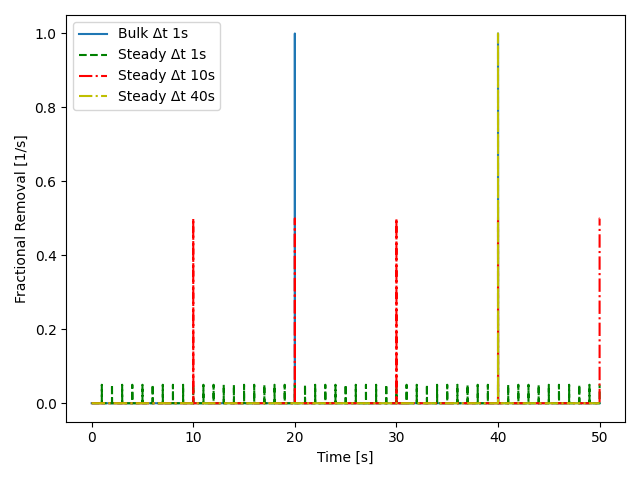
\includegraphics[scale=0.45]{images/bulk-compare-cycles.png}
  \caption{Plot showing how bulk and steady batchwise reprocessing removal works as a function of time for an example with a cycle time of 20 seconds.}
   \label{fig:bulk_repr_cnst}
\end{figure}

Figure \ref{fig:bulk_repr_cnst} shows an example fractional removal scheme for a fission product with a cycle time of 20 seconds. The Bulk method simply extracts 100\% of the product every 20 seconds, no matter how small the depletion step size is. The steady method removes some fraction every depletion step, which allows a semi-continuous process as the depletion step size becomes smaller and smaller. This can be seen in how a 10 second depletion step results in 50\% removal every 10 seconds, whereas a 1 second step allows for 5\% removal per depletion step.


% Add comparison of batch/steady for matrix of possible combinations. 

\begin{figure}[H]
  \centering
  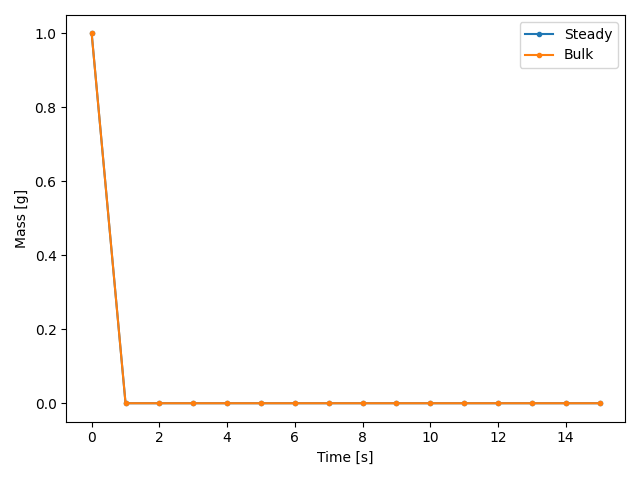
\includegraphics[scale=0.45]{images/batch-steady-identical-compare.png}
  \caption{Plot showing how bulk and steady batchwise reprocessing are identical while the cycle time is shorter than or equal to the depletion step size.}
   \label{fig:bulk_repr_comp}
\end{figure}

A useful piece of information to note is that if the cycle time is shorter than or equal to the depletion step size, then the steady and bulk batchwise methods will be identical to each other, as demonstrated in Figure \ref{fig:bulk_repr_comp} which shows a simple model case with 1 second depletion steps and 1 second cycle times for an imaginary isotope. For the MSBR simulation, this means that the noble metals, gasses, and protactinium reprocessing will remain the same for either batchwise method employed. However, the longer cycle time groups such as the rare earths and volatile fluorides have cycle times which are 10-20 times longer than the depletion step size. Figure \ref{fig:bulk_repr_diff} shows a simulation of this for a situation where an isotope is generated at a rate of 1 gram per second, and is simulated with some combination of cycle time and depletion step size where the depletion step size is smaller than the cycle time.

\begin{figure}[H]
  \centering
  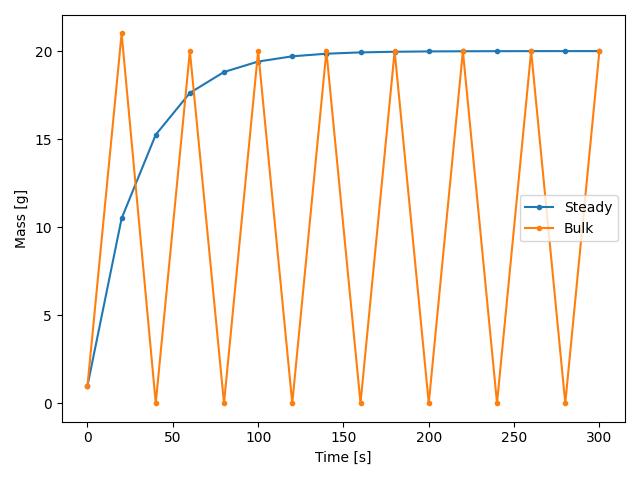
\includegraphics[scale=0.45]{images/batch-40-20.png}
  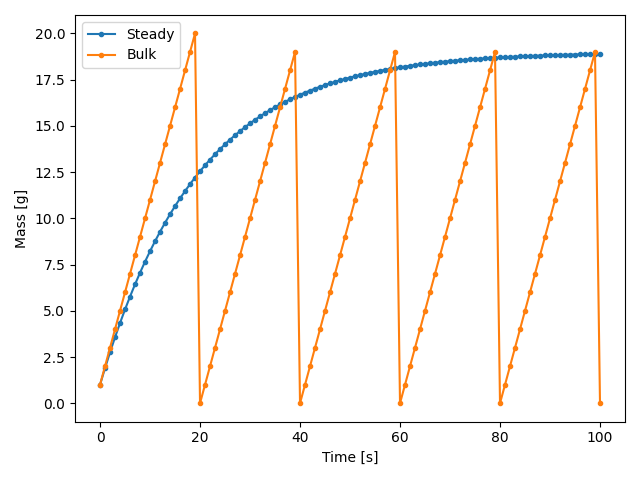
\includegraphics[scale=0.45]{images/batch-20-1.png}
  \caption{Plot showing how bulk and steady batchwise reprocessing are different while the cycle time is longer than the depletion step size for a 40 second cycle time and 20 second depletion step (top) and a 20 second cycle time with a 1 second depletion step (bottom).}
   \label{fig:bulk_repr_diff}
\end{figure}

One interesting aspect to note from this figure is that the steady method approaches a steady state value which is at the peak of the bulk method. This result can be confirmed by checking that the solutions for both the steady and bulk methods are valid. To check the solution, the 40 second cycle time and 20 second depletion step will be used. 

For the bulk method, after 100\% removal after the first cycle time, or 40 seconds, the mass then oscillates between 20 and 0 grams. This makes sense since 20 grams are generated over 20 seconds while every 40 seconds there is 100\% removal. 

For the steady method, the initial mass of 1 gram gains 20 grams over 20 seconds, yielding 21 grams. However, the steady removal then requires removal of 50\%, previously discussed and shown in Figure \ref{fig:bulk_repr_cnst}. This 50\% removal then drops the mass to 10.5 grams. 20 more grams are added to this value and 50\% is removed again, continuing iteratively. This can then be re-written as an infinite sum in order to determine the steady state solution. The first three iterations are shown in Equations \eqref{eq:ss-mass-p1} and \eqref{eq:ss-mass-p2}, where the value of 20 is the mass added during each depletion step and the value of 0.5 is the fractional removal performed each depletion step.

\begin{equation} \hfill 
m_{ss} = (((N_0+20)(0.5)+20)(0.5)+20)(0.5)
\hfill\label{eq:ss-mass-p1} \end{equation}

\begin{equation} \hfill 
m_{ss} = 0.5^3 N_0 + 0.5^3 (20) + 0.5^2 (20) + 0.5 (20)
\hfill\label{eq:ss-mass-p2} \end{equation}

Continuing this form infinitely yields Equation \eqref{eq:ss-mass-p3}, where the infinite sum yields 1, resulting in a net value of 20, the result of which is unaffected by the initial mass of the isotope and instead depends on the generation and reprocessing rates.

\begin{equation} \hfill 
m_{ss} = 20 \sum_{n=1}^\infty \frac{1}{2}^n 
\hfill\label{eq:ss-mass-p3} \end{equation}

% Add generic form (x added per second, y removal rate)

Overall, this shows that the steady and bulk batchwise methods have some similarities, but for elements with longer cycle times, the bulk method will experience oscillations whereas the steady method will level off smoothly.

\section{Continuous Reprocessing}

The continuous reprocessing functionality of Serpent2 was undocumented for several years aside from on the Serpent2 forums, but more recently work has gone into providing documentation. However, there has not been comparisons of Serpent2 continuous reprocessing with Serpent2 batchwise reprocessing with no differences between the models aside from the mathematical reprocessing approach used.

There are three different options which can be used for the Serpent2 built-in continuous reprocessing. The different options are defined in Serpent2 as 0, 1, and 2; which are henceforth referenced as Constant, Decay, and Step reprocessing. These names are selected because they closely describe the behaviour of each of the methods.

\subsection{Constant}
The Constant reprocessing method is the only method of the three options which does not conserve mass. This option instead generates mass the same way as the Decay reprocessing method for the initial step, then continues using that mass rate from that point onwards.

This method is useful for handling a constant fresh fuel feed rate, or any other situation where a constant addition of mass is desired. Because this method does not remove mass, it is not useful for any sort of constant removal.
%The main issue with this method is that it, for Serpent 2.32.1, it causes depletion to cease functioning while this method is active. This is an issue, since for most cases where a user wants to incorporate a feed rate, depletion is being considered.

\subsection{Decay}
The Decay reprocessing method is the most useful of the three options, and that is due to its flexibility in its usefulness. This method adds a decay term to whatever material it is attached to, and that decay term becomes a feed term to whatever material is set to receive the flow. For fission product removal, this is likely some material which is not modeled in the geometry of the problem but only exists to receive the fission product waste. However, this term can instead be leveraged to turn it into a feed rate.

This can be performed by attaching the decay term to a material which contains a volume of the desired feed, and then having that material feed into the core. The feed then "decays" from the feed tank into the core, essentially operating as a feed. Using this same method but altering the reprocessing constant or volume of the feed tank allows for an essentially constant feed rate, where the removed mass is negligible compared to the net mass.

Additionally, for this method, there are multiple approaches which can be used to calculate the reprocessing constants that should be implemented. These approaches are named "Cycle Time Decay", "Cycle Rate", and "SaltProc Cycle Rate" accordingly. The Cycle Time Decay approach treats the cycle time as if it is twice a half-life, and the cycle time is an exponential process. The Cycle Rate approach treats the cycle time as the time where 100\% of removal occurs, and then linearly extrapolates by assuming an equal percentage removal occurs up to that point.

The reason these approaches are implemented is because molten salt reactor reprocessing schemes provide reprocessing data in terms of cycle times. The cycle time is the amount of time it takes for a given element to be removed from the system. This cannot be directly solved using the Bateman equation, as shown in Equations \eqref{eq:decay_1} through \eqref{eq:decay_3} and \eqref{eq:decay_4} through \eqref{eq:decay_7}. 

\begin{equation} \hfill
\frac{dN}{dt} = -\lambda_r N
\hfill\label{eq:decay_1} \end{equation}

\begin{equation} \hfill
N(\tau) = 0 = N_0 e^{-\lambda_r \tau}
\hfill\label{eq:decay_2} \end{equation}

\begin{equation} \hfill
-ln(0) = \lambda_r \tau
\hfill\label{eq:decay_3} \end{equation}

Equations \eqref{eq:decay_1} through \eqref{eq:decay_3} show how the solution results in a reprocessing constant of infinity when only continuous removal is considered.

\begin{equation} \hfill
\frac{dN}{dt} = C -\lambda_r N
\hfill\label{eq:decay_4} \end{equation}

\begin{equation} \hfill
N(\tau) = 0 = N_0 e^{-\lambda_r \tau} + \frac{C}{\lambda_r} \left( 1 - e^{-\lambda_r \tau} \right)
\hfill\label{eq:decay_5} \end{equation}

\begin{equation} \hfill
0 = N_0 e^{-\lambda_r \tau} + \frac{C}{\lambda_r} - \frac{C}{\lambda_r} e^{-\lambda_r \tau}
\hfill\label{eq:decay_6} \end{equation}

\begin{equation} \hfill
0 = \lambda_r N_0 e^{-\lambda_r \tau} + C - C e^{-\lambda_r \tau}
\hfill\label{eq:decay_7} \end{equation}


 Equations \eqref{eq:decay_4} through \eqref{eq:decay_7} show that the only real solution to a steady accumulation and continuous removal is with a reprocessing constant of 0. 

\subsubsection{Cycle Time Decay}

The Cycle Time Decay approach is a simple method which makes use of the mathematical form of the Decay reprocessing method. Because it adds a "decay-like" term to the Bateman equation, this approach takes the cycle time for the target, cuts it in half, and then treats that value as the reprocessing half-life for that target. This process is shown in Equations \eqref{eq:ctd_1} and \eqref{eq:ctd_2}.

\begin{equation} \hfill
\tau_{1/2} = \frac{T_{cyc}}{2}
\hfill\label{eq:ctd_1} \end{equation}

\begin{equation} \hfill
\lambda_r = \frac{ln(2)}{\tau_{1/2}}
\hfill\label{eq:ctd_2} \end{equation}

%An example of how this approach is mathematically modeled can be seen in Figure \ref{fig:ctd_examp}.

%\begin{figure}[H]
%  \centering
%  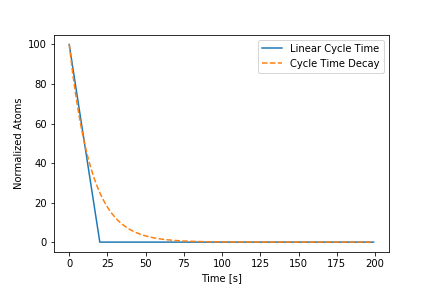
\includegraphics[scale=0.6]{images/Cycle_Time_Decay_example_0.png}
%  \caption{A comparison between a linear 20 second cycle time and the Cycle Time Decay approach.}
%   \label{fig:ctd_examp}
%\end{figure}

%It can be seen in this figure that this approach is accurate in being close to the cycle time, though this accuracy is limited to above approximately 40\% of the atoms. Because fission products are continuously generated though, it is expected to be within the more accurate regions.
%Figure \ref{fig:ctd_examples} shows how the Cycle Time Decay approach fares when accumulation of fission products is incorporated into the problem. 

%\begin{figure}[H]
%  \centering
%  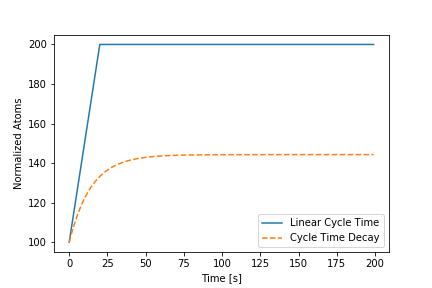
\includegraphics[scale=0.6]{images/Cycle_Time_Decay_example_10.png}
%  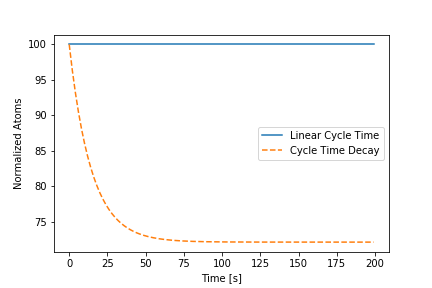
\includegraphics[scale=0.6]{images/Cycle_Time_Decay_example_5.png}
%  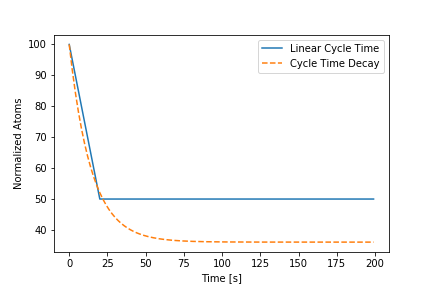
\includegraphics[scale=0.6]{images/Cycle_Time_Decay_example_2.5.png}
%  \caption{Comparison with linear 20 second cycle time and Cycle Time Decay approach for 10, 5, and 2.5 %atoms per second accumulation, respectively.}
%   \label{fig:ctd_examples}
%\end{figure}

%The top plot of Figure \ref{fig:ctd_examples} shows a situation where the accumulation of fission products occurs at a higher rate than the cycle time, leading to a larger steady-state value than initially present. The Cycle Time Decay does not reach the 200 value and instead is lower at 144. The middle plot shows a situation where the accumulation rate matches the cycle time removal rate, the same rate that the linear cycle time would have them removed, resulting in a steady-state value. However, the Cycle Time Decay approach drops to approximately 72 levels off. The bottom plot shows an accumulation which is half the linear cycle time removal rate. These results are somewhat close, though the Cycle Time Decay does not reach the same steady-state value, instead stabilizing around 40 instead of 50. For various accumulation rates ranging from 0.1 to 1 million atoms per second, the steady-state difference comes out to approximately 27.86\% for each. This percent difference also stays the same for different cycle times as well.

An example of implementing this approach for a 30 second cycle time would then have a 15 second reprocessing half-life. This is then converted to a reprocessing constant in the same way that a decay half-life is converted to a decay constant, which can be seen in Equation \eqref{eq:ctd_eqn}, resulting in a value of 0.0462 $s^{-1}$.

\begin{equation} \hfill
\lambda_{r} = \frac{ln(2)}{15} = 0.0462 s^{-1}
\hfill\label{eq:ctd_eqn} \end{equation}

\subsubsection{SaltProc Cycle Time Decay}

This approach is the same as Cycle Time Decay, but alters for any target which has a cycle time less than the batchwise reprocessing step incorporated by SaltProc. For example, a 3 day cycle time for some target would be treated the same as the standard Cycle Time Decay. However, a cycle time shorter than the 3 day batchwise reprocessing step used by SaltProc for the MSBR has its half-life extended to the SaltProc minimum value of 1.5 days. For example, a 30 second cycle time would instead be treated as a 3 day cycle time, which would result in a half-life of 1.5 days. Plugging in, this would result in a reprocessing constant of 0.462 $days^{-1}$, or 5.348E-6 $s^{-1}$. This is the reprocessing constant for any cycle time which is less than or equal to three days. 

\subsubsection{Cycle Rate}

The Cycle Rate approach uses a linear approximation such that the inverse of the cycle time is the rate at which material is removed. This is represented by, for example, 10\% removal per second would neglect the efficiency decrease over time and give 100\% removal after 10 seconds. This is calculated by investigating a unit time progression, i.e. 1 second or 1 day. Over this time period, the removal of atoms should be the fractional rate value, which means the final atom count at a time of 1 should be 1 - $X$, where $X$ is the fractional removal rate. This can be seen in Equations \eqref{eq:nat_log_0} and \eqref{eq:nat_log_3}.

\begin{equation} \hfill
X = \frac{1}{T_{cyc}}
\hfill\label{eq:nat_log_0} \end{equation}

\begin{equation} \hfill
\frac{dN}{dt} = -\lambda_r N
\hfill\label{eq:nat_log_1} \end{equation}

\begin{equation} \hfill
N(t) = N_0 e^{-\lambda_r t}
\hfill\label{eq:nat_log_1} \end{equation}

\begin{equation} \hfill
N(t = 1) = (1-X) N_{0}
\hfill\label{eq:nat_log_2} \end{equation}

\begin{equation} \hfill
(1-X) N_{0} = N_{0} e^{-\lambda_r (1)}
\hfill\label{eq:nat_log_2_1} \end{equation}

\begin{equation} \hfill
-ln(1-X)  = \lambda_r
\hfill\label{eq:nat_log_2_5} \end{equation}

\begin{equation} \hfill
\lambda_r = ln\left( \frac{1}{1-X} \right)
\hfill\label{eq:nat_log_3} \end{equation}

However, the mathematical model actually results in exponential decay in the removal effectiveness due to a decreasing amount of the target to remove. %Figure \ref{fig:cr_examp} shows how this approach compares to the actual exponential decay.

%\begin{figure}[H]
%  \centering
%  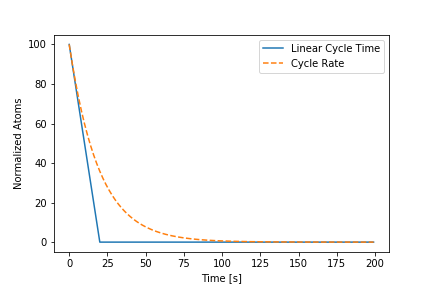
\includegraphics[scale=0.6]{images/Cycle_Rate_example_0.png}
%  \caption{A comparison between a linear 20 second cycle time and the Cycle Rate approach.}
%   \label{fig:cr_examp}
%\end{figure}

%It can be seen from this figure that the Cycle Rate approach removes at a rate sufficient to match the cycle time of 20 seconds while there are ~60\% of the atoms present. Once the atom count drops, the removal becomes less effective however, which is physical but makes the model less effective at matching the cycle time. Because the Cycle Rate approach is used on fission products which are being constantly generated, the difference is expected to be fairly small.

%\begin{figure}[H]
%  \centering
%  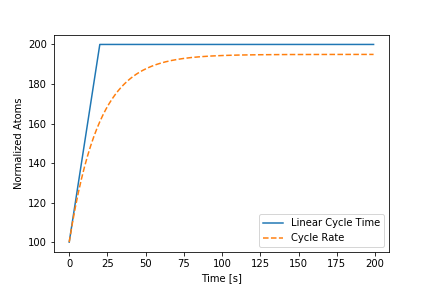
\includegraphics[scale=0.6]{images/Cycle_Rate_example_10.png}
%  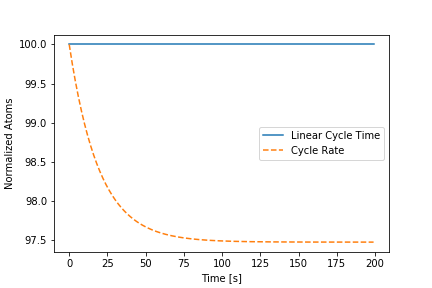
\includegraphics[scale=0.6]{images/Cycle_Rate_example_5.png}
%  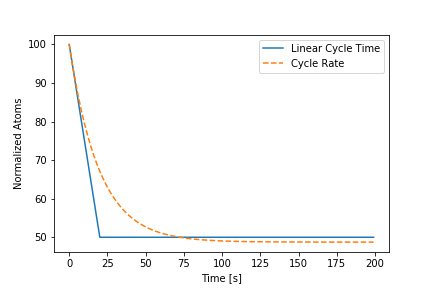
\includegraphics[scale=0.6]{images/Cycle_Rate_example_2.5.png}
%  \caption{Comparison with linear 20 second cycle time and Cycle Rate approach for 10, 5, and 2.5 atoms %per second accumulation, respectively.}
%   \label{fig:cr_examples}
%\end{figure}



An example cycle time of 30 seconds would be modeled by taking the inverse, which gives 0.033 $s^{-1}$. This value is then converted to a reprocessing constant by plugging it into the solved differential equation form shown in Equations \eqref{eq:cr_exmp1} and \eqref{eq:cr_eqn}, giving a value of 0.0339 $s^{-1}$.

\begin{equation} \hfill
X = \frac{1}{30} = 3.33E\minus2 s^{-1}
\hfill\label{eq:cr_exmp1} \end{equation}

\begin{equation} \hfill
\lambda_{r} = ln\left(\frac{1}{1 - 3.33E\minus2}\right) = 0.0339 s^{-1}
\hfill\label{eq:cr_eqn} \end{equation}

%The reason this approach is used is two-fold. Firstly, SaltProc v0.3 uses the same linear fractional removal approximation for its batchwise removal, so this same method is employed to better compare the two models. Secondly, due to the mathematical nature of the Decay reprocessing model, 100\% removal only occurs for a reprocessing constant of infinity. This means an approximation must be made. This is also a reasonable approximation since there is constant addition of material, meaning that the exponential line and the linear line are not going to be significantly different.


\subsubsection{SaltProc Cycle Rate}

The SaltProc Cycle Rate approach is the same as the Cycle Rate approach, but takes into account the limiting nature of the 3 day batchwise reprocessing step used by SaltProc. For example, a 6 day cycle time target would be modeled the same using the SaltProc Cycle Rate approach as the standard Cycle Rate approach. However, anything shorter than 3 days would be modeled differently, since that is the batchwise reprocessing step inocorporated by SaltProc for modeling the MSBR. For example, a 30 second cycle time would be analyzed instead as a 3 day cycle time, since SaltProc can only remove 100\% of material after a minimum of 3 days. This means the inverse would be 0.333 $days^{-1}$, or 3.858E-4 $s^{-1}$. Converting to a reprocessing constant gives a value of 3.858E-6 $s^{-1}$. This is the reprocessing constant for any cycle time which is less than or equal to three days.

\subsubsection{Direct Linear Approach}

Another approach is to directly apply the Cycle Rate removal rate, which is the inverse of the cycle time, as the reprocessing constant \cite{hombourger_eql0d_2020}. This is referred to as the Direct Linear approach. This approach is similar to the Cycle Rate approach, though the derivation for it is slightly different. This can be seen in Equations \eqref{eq:dir_lin_0} through \eqref{eq:dir_lin_10}, where Equations \eqref{eq:dir_lin_8} and \eqref{eq:dir_lin_9} uses L'Hôpital's rule.

\begin{equation} \hfill
X = \frac{1}{T_{cyc}}
\hfill\label{eq:dir_lin_0} \end{equation}

\begin{equation} \hfill
\frac{dN}{dt} = -\lambda_r N
\hfill\label{eq:dir_lin_1} \end{equation}

\begin{equation} \hfill
N(t) = N_0 e^{-\lambda_r t}
\hfill\label{eq:dir_lin_1_2} \end{equation}

\begin{equation} \hfill
N_{cur} = N_{prev} e^{-\lambda_r \Delta t}
\hfill\label{eq:dir_lin_2} \end{equation}

\begin{equation} \hfill
N_{cur} = (1 - \Delta t X) N_{prev}
\hfill\label{eq:dir_lin_3} \end{equation}

\begin{equation} \hfill
(1 - \Delta t X) N_{prev} = N_{prev} e^{-\lambda_r \Delta t}
\hfill\label{eq:dir_lin_4} \end{equation}

\begin{equation} \hfill
-ln\left((1 - \Delta t X)\right) = \lambda_r \Delta t
\hfill\label{eq:dir_lin_5} \end{equation}

\begin{equation} \hfill
\lambda_r = \frac{-ln\left((1 - \Delta t X)\right)}{\Delta t}
\hfill\label{eq:dir_lin_6} \end{equation}

\begin{equation} \hfill
\lambda_r = lim_{\Delta t \to 0} \frac{-ln\left((1 - \Delta t X)\right)}{\Delta t}
\hfill\label{eq:dir_lin_7} \end{equation}

\begin{equation} \hfill
\lambda_r = \frac{0}{0}
\hfill\label{eq:dir_lin_8} \end{equation}

\begin{equation} \hfill
\lambda_r = lim_{\Delta t \to 0} \frac{X}{1-X\Delta t}
\hfill\label{eq:dir_lin_9} \end{equation}

\begin{equation} \hfill
\lambda_r = X = \frac{1}{T_{cyc}}
\hfill\label{eq:dir_lin_10} \end{equation}

These equations follow a similar path to the Cycle Rate approach, but instead of using the linear approximation value after a unit time step, this approach generates the reprocessing constant while implementing the linear approximation as the time step goes to zero.

The differences between Cycle Rate and Direct Linear approaches can be seen in Table \ref{tab:repr_decay_view}, where for longer cycle times, the difference is negligible, but for shorter cycle times, the difference becomes larger. However, since extremely short cycle times are not realistically practical, the two approaches are approximately equivalent. Overall, the Direct Linear approach is more numerically stable, however, since it does not have asymptotic until reaching a cycle time of 0 seconds, whereas the Cycle Rate method has asymptotic behaviour at 1 second cycle time. This can be seen in Figure \ref{fig:dl_cr_asymptotic}. The asymptotic behaviour for a 0 second cycle time is not an issue because there are no negative cycle times, meaning the value is only approached from the positive side and behaves as physically expected.

\begin{table}[H]
\renewcommand{\arraystretch}{1.25}
\caption{Decay Reprocessing Approaches}
\label{tab:repr_decay_view}
\begin{center}
\begin{tabular}{ | c | c | c | c | c | }
 \hline
 Cycle Time & Removal Rate [$s^{-1}$] & CR $\lambda_{r}$ [$s^{-1}$] & DL $\lambda_{r}$ [$s^{-1}$] & $\Delta \lambda_{r}$\\
 \hline
 \hline
 3 d & 3.86E-6 & 3.86E-6 & 3.86E-6 & 7.44E-12\\
 20 s & 0.05 & 5.13E-2 & 5.00E-2 & 1.29E-3\\
 5 s & 0.2 & 2.23E-1 & 2.00E-1 & 2.31E-2\\
 2 s & 0.5 & 6.93E-1 & 5.00E-1 & 1.93E-1\\
 1 s & 1 & - & 1 & -\\
 \hline
\end{tabular}
\end{center}
\end{table}

\begin{figure}[H]
  \centering
  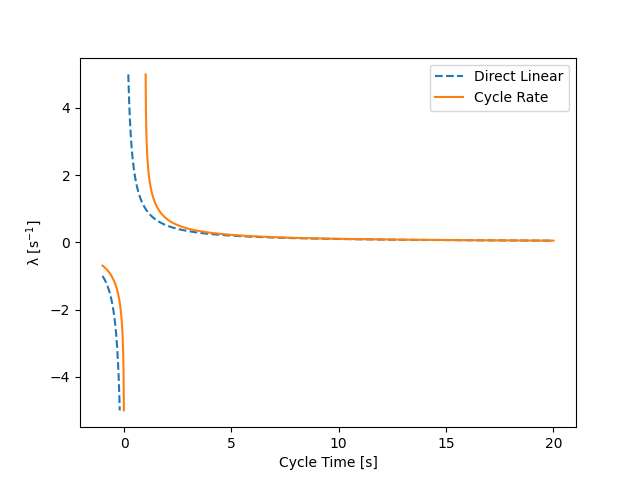
\includegraphics[scale=0.55]{images/dl_cr_asymptote.png}
  \caption{A comparison of the Direct Linear and Cycle Rate reprocessing constants for different cycle times.}
   \label{fig:dl_cr_asymptotic}
\end{figure}

Because the shortest cycle time for the MSBR is 20 seconds, this shows that the Cycle Rate and Directly Linear approaches are roughly equivalent for this reprocessing scheme.

%Figure \ref{fig:dl_cr_compare_linear} shows the implementation of both methods for an example nuclide with a cycle time of CYCLE TIME and an accumulation rate of ACCUMULATION RATE. It can be seen from this figure how the Direct Linear and Cycle Rate approaches differ in modeling of the same isotope.

%\begin{figure}[H]
%  \centering
%  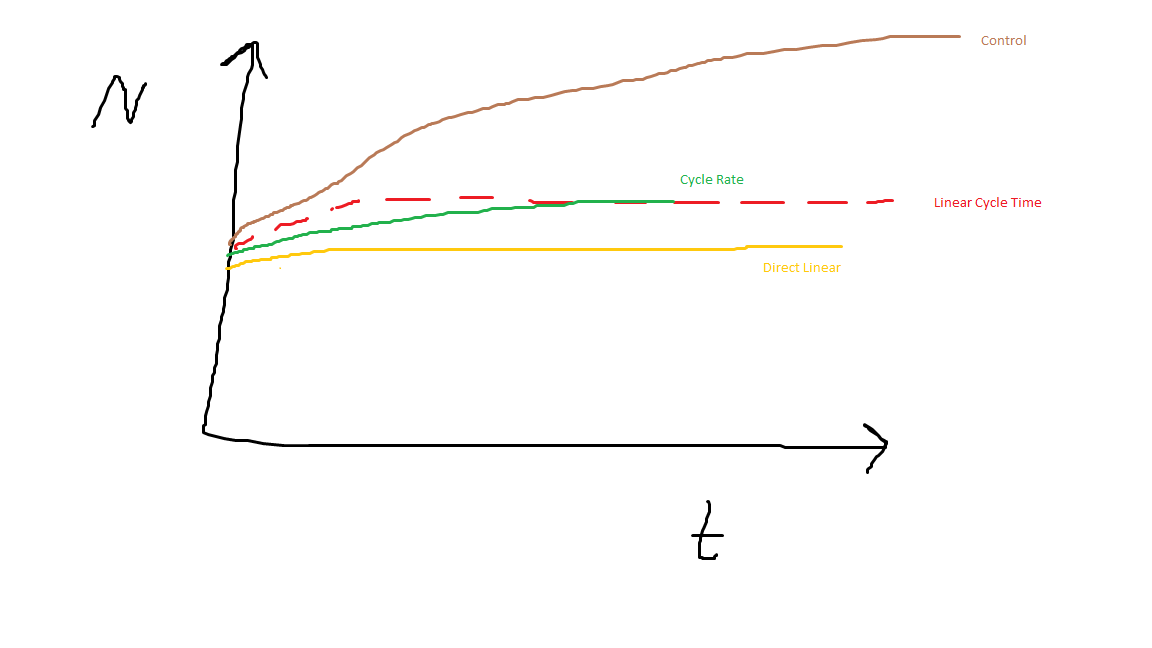
\includegraphics[scale=0.25]{images/direct_linear_compare.png}
%  \caption{A comparison of the Direct Linear and Cycle Rate approaches for a particular element with a %given accumulation rate and cycle time(s).}
%   \label{fig:dl_cr_compare_linear}
%\end{figure}


\subsubsection{Decay Approaches Summary}

Figure \ref{fig:repr_cnst} shows how the reprocessing constants for the different approaches vary as a function of cycle time.

\begin{figure}[H]
  \centering
  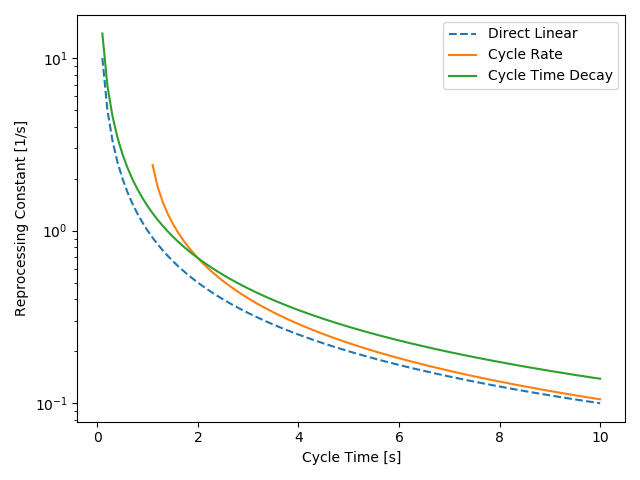
\includegraphics[scale=0.45]{images/cont-compare-cycles.png}
  \caption{Plot of how reprocessing constants for different approaches vary with cycle time.}
   \label{fig:repr_cnst}
\end{figure}

Figure \ref{fig:repr_cnst} shows the three different continuous decay based methods for reprocessing as a function of various cycle times. From the figure, it can be seen that the Cycle Rate method does not have results for cycle times less than or equal to 1 second, which is a significant weakness of the method since physical processes could exist with a cycle time in that range. The other two methods provide results down to a 0 second cycle time, which allows full coverage of possible cycle time values.

The Direct Linear method behaves similarly to the Cycle Time Decay method during small cycle times and the Cycle Rate method for longer cycle times. This is due to the general form of the equations for each, where at small cycle times the inverse cycle time relationship with the Cycle Time Decay method dominates, while at larger cycle times the Cycle Rate log of the inverse term matches more closely.

%WHICH IS THE MORE ACCURATE APPROACH AMONG THE THREE (There isn't a way to validate this without more information on how cycle time is generated. Perhaps if instead we find data for molten salt reprocessing and compare against that it might be useful?) (Maybe check average net atoms for steady and bulk batch and compare, then maybe check a comparison of net atoms at 1/2 cycle time and cycle time, etc.)

%CITE "Liquid Fuel Molten Salt Reactors for Thorium Utilization" This paper uses bulk batchwise reprocessing

%INCLUDE PLOT OF N(t) FOR DIFFERENT CYCLE TIMES WHERE ONLY INITIAL MASS AND REPROCESSING ARE CONSIDERED. (DIRECT LINEAR AND CYCLE RATE ARE THE SAME FOR LARGE CYCLE TIMES)

%REPLICATE ATOMS OVER TIME PLOTS FOR DIFFERENT MODELS AND DIFFERENT ACCUMULATION RATES TO SEE HOW STEADY-STATE VALUES COMPARE.

\subsection{Step}

The Step reprocessing method implemented in Serpent2 is mathematically very similar to the Decay model, but instead of updating continuously in time, it instead is updated during new depletion steps. In this manner, it is a sort of mix between the Constant method and the Decay method. This is because over a single depletion step, it is a constant added or subtracted from the Bateman equation, while over many depletion steps, it follows the same exponential decay form of the Decay method.

This particular method is not useful for extracting fission products, and is not needed for constant feed rates since that can be modeled using the Decay method. This method could be useful for inducing a step drop in feed rate, though this would require running only a single depletion step until the drop occurred. Additionally, this drop could be simulated by running the Decay method and reducing the reprocessing constant. This would allow for flexibility in the distribution of depletion steps as well without having to worry about changing the behaviour of the reprocessing functionality. 

Another potential issue with the Step method is that the depletion step can last long enough that the constant mass removal causes the mass to go negative. However, Serpent2 will cease running if this occurs. The Decay method does not mathematically allow for negative mass, the Constant method does not conserve mass, and the Step method stops running once there is negative mass.

The main potential use of the Step reprocessing may be for movement of material at a set rate. This could be implemented by writing a script to check the current number of atoms of the target and adjusting the reprocessing rate accordingly. However, for the MSBR, this form of reprocessing is not necessary, and is thus not implemented.

\section{Mass Balancing}

One of the useful features of batchwise reprocessing is that the net mass of the core can be balanced by adjusting the feed rates to provide the same amount into the core that is removed through reprocessing. Alternative methods also exist, such as removing excess mass or increasing the volume \cite{ridley_method_2017}. SaltProc version 0.1 does not account for mass balancing but maintains a constant thorium mass, whereas SaltProc version 0.3 has the feed rates set to maintain mass. Mass balancing is particularly important in Serpent2 due to the way masses in Serpent2 are handled.

In Serpent2, an increase in mass does not affect volume, but instead increases the density of that isotope in the material accordingly. This affects macroscopic cross section calculations, and can lead to variation in results if not accounted for, since in reality volumetric expansion could be assumed. Though there are several methods to handle mass balancing with a batch method, it not currently continuously possible in Serpent2.

In order to balance the mass in Serpent2 continuously, one approach could be to iteratively perform depletion calculations while updating feed rates until a balanced mass is found while also minimizing some other parameter, such as net mass of material added. However, the current reprocessing options available in Serpent2 only allows for pseudo-constant and decaying feed rates over the depletion step. With those two feed types available, it is not possible to have a constant mass balance.

It is possible to have the masses at the end of each depletion step remain constant, but this does handle mass fluctuations during depletion. It does, however, solve the issue of the density variation causing a difference in cross sections.

Overall, if the net mass difference is sufficiently small, it does not have to be considered since the results would not be significantly impacted. To check this for the MSBR, a simple back-of-the-envelope calculation can be used. To determine the maximum possible increase in density, the mass loss due to fission and reprocessing is neglected, and only mass addition from the thorium feed rate is considered. The uranium feed is not added because it is equivalent to the protactinium removal, so it would have a negligible impact on net mass. 

\begin{equation} \hfill
\Delta m = \Dot{m}_{feed} \Delta t \approx (2.5)(6000) = 15,000 kg
\hfill\label{eq:m_gain} \end{equation}

It can be seen in Equation \eqref{eq:m_gain} that the net mass gain for an average feed rate of 2.5 kilograms per day over 6000 days is 15,000 kg \cite{rykhlevskii_fuel_2020, betzler_molten_2017}. This does seem to be a very large value, but the importance of the mass in the depletion calculation is primarily in how it affects cross sections, which means that the impact on the overall thorium density is important. The thorium density is 1.46 grams per cubic centimeter, and the net volume is approximately 48.71 cubic meters. The density with the added mass is calculated using Equation \eqref{eq:new_rho}.

\begin{equation} \hfill
\rho_f = \frac{m_0 + \Delta m}{V} = \frac{(4.871E7)(1.45919E\minus3) + (15,000)}{4.871E7} 
\hfill\label{eq:new_rho} \end{equation}

The final density comes out to be 1.767 grams per cubic centimeter, which is a percent difference of ~21\%. Although this is an upper bound on the mass difference, a 21\% difference in the expected cross section would result in significant error in the results. Therefore, since it is possible for the mass balancing to have an impact, it should be investigated to ensure the mass balancing is not impacting the results in any unexpected manner.

%DIFFERENT FEED RATE VARIANTS IMPLEMENTED

%MSBR MASS BALANCE BATCH AND CONTINUOUS


%\section{Uncertainty}

%SHANNON ENTROPY

%STOCHASTIC ERROR VS ACTUAL DIFFERENCE IN RESULTS

%DEPLETION ERROR BUILDUP

%\section{Continuous Reprocessing Implementation}

\section{Effects of Delayed Neutrons on Depletion}

Delayed neutrons have a softer energy spectrum and drift along with the movement of the fuel salt in a fluid fueled molten salt reactor. This means that the delayed neutron precursors, of which some fraction leave the core and some move to less neutron important regions, have the potential to alter the depletion results of the MSBR model.

However, it has been shown by Zhou et al that for the MSBR, the delayed neutron precursor drift has a negligible impact on depletion results \cite{zhou_fuel_2018}. Although Zhou et al has shown this, it is still worth considering the maximum possible effect delayed neutron precursors could have on depletion results. In order to determine this, the Serpent2 functionality of disabling delayed neutrons is employed \cite{leppanen_serpent_2015}. Using this method, two different models are generated of the MSBR. The first is one in which the delayed neutron precursors are evenly distributed within the core, which is the model implemented by SaltProc and this work \cite{rykhlevskii_modeling_2019}. The second model is one in which delayed neutrons no longer exist. This is beyond the greatest effects the delayed neutron precursor drift could have on depletion, so the absolute maximum effect of delayed neutron precursors on depletion results can be determined.

Because the delayed neutron precursors are fission products or come from the decay of fission products, depletion must be performed. For reprocessing, the average feed rate from SaltProc is used with continuous Direct Linear reprocessing, while Direct Linear reprocessing is used for fission product removal. 

The impact on $k_{eff}$ was investigated, and it was determined that the delayed neutrons from fission products add roughly 20 pcm to $k_{eff}$ after 6,000 days of operation, which is roughly steady state operation. The masses of various isotopes, such as uranium-235 and thorium-232, were also compared, though no statistically significant difference was found. Therefore, the net impact of delayed neutrons from fission product precursors is negligible on depletion results, which agrees with the results from Zhou et al.

%Figure \ref{fig:keff_compare} shows how the multiplication factors evolve over time. The final difference between the two values is FINALDIFF.

%\begin{figure}[H]
%  \centering
%  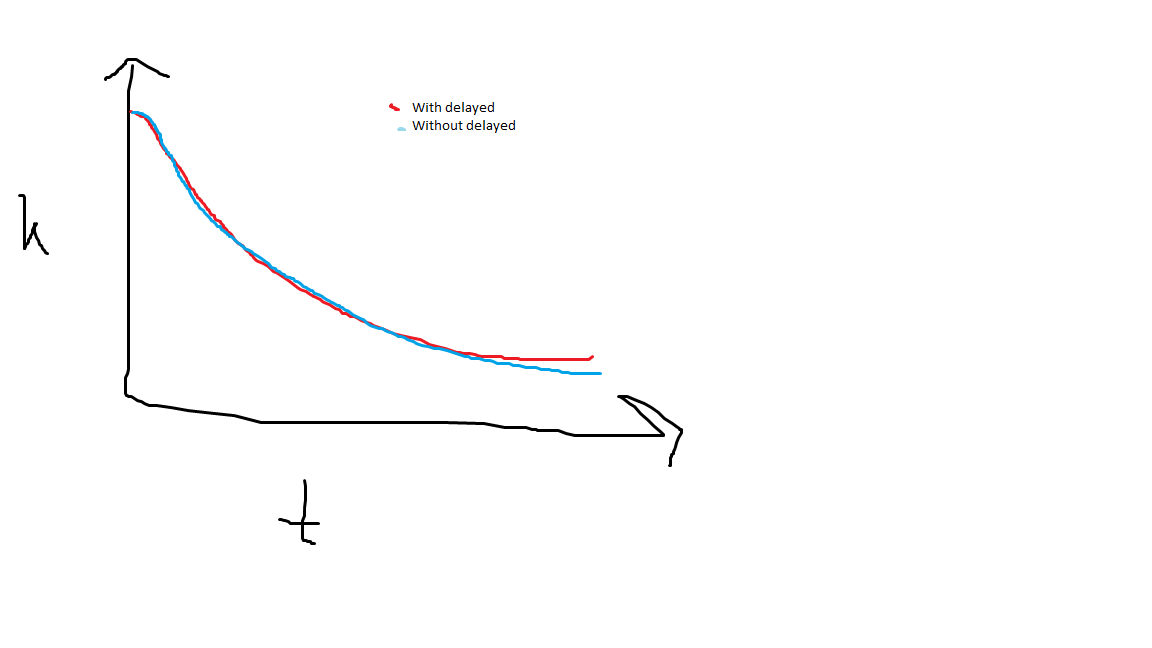
\includegraphics[scale=0.45]{images/keff_dnp_compare.png}
%  \caption{Comparison of $k_{eff}$ over time with and without delayed neutrons.}
%   \label{fig:keff_compare}
%\end{figure}

%PLOT OF SPECTRUMS WITH AND WITHOUT DELAYED NEUTRONS

%TABLE OF IMPORTANT ISOTOPE CONCENTRATIONS FOR WITH AND WITHOUT





% Toggle remove this for debugging
%\nocite{*}


\section{Serpent MSBR Model}

The results generated in this work come from the MSBR, particularly the model developed by Rykhlevskii \cite{rykhlevskii_advanced_2018}. The geometry of the model has remained unchanged, while the reprocessing has been overhauled using the continuous reprocessing functionality in Serpent2 which was previously undocumented. Previously, SaltProc's batchwise reprocessing was used, but the continuous reprocessing in Serpent2 is incorporated in this work.

\subsection{Reprocessing Structure}

There are two different reprocessing schemes developed in this work. Both schemes follow the MSBR reprocessing scheme, and vary how refueling functions. The first method matches the method of Rykhlevskii, where the uranium-233 feed is treated as equivalent to the protactinium-233 removal rate. In this case, the average uranium-233 feed rate from Rykhlevskii is used over the entire simulation time \cite{rykhlevskii_advanced_2018}. A simplified overview of this scheme can be seen in Figure \ref{fig:spmatchrepr}.


\begin{figure}[H]
  \centering
  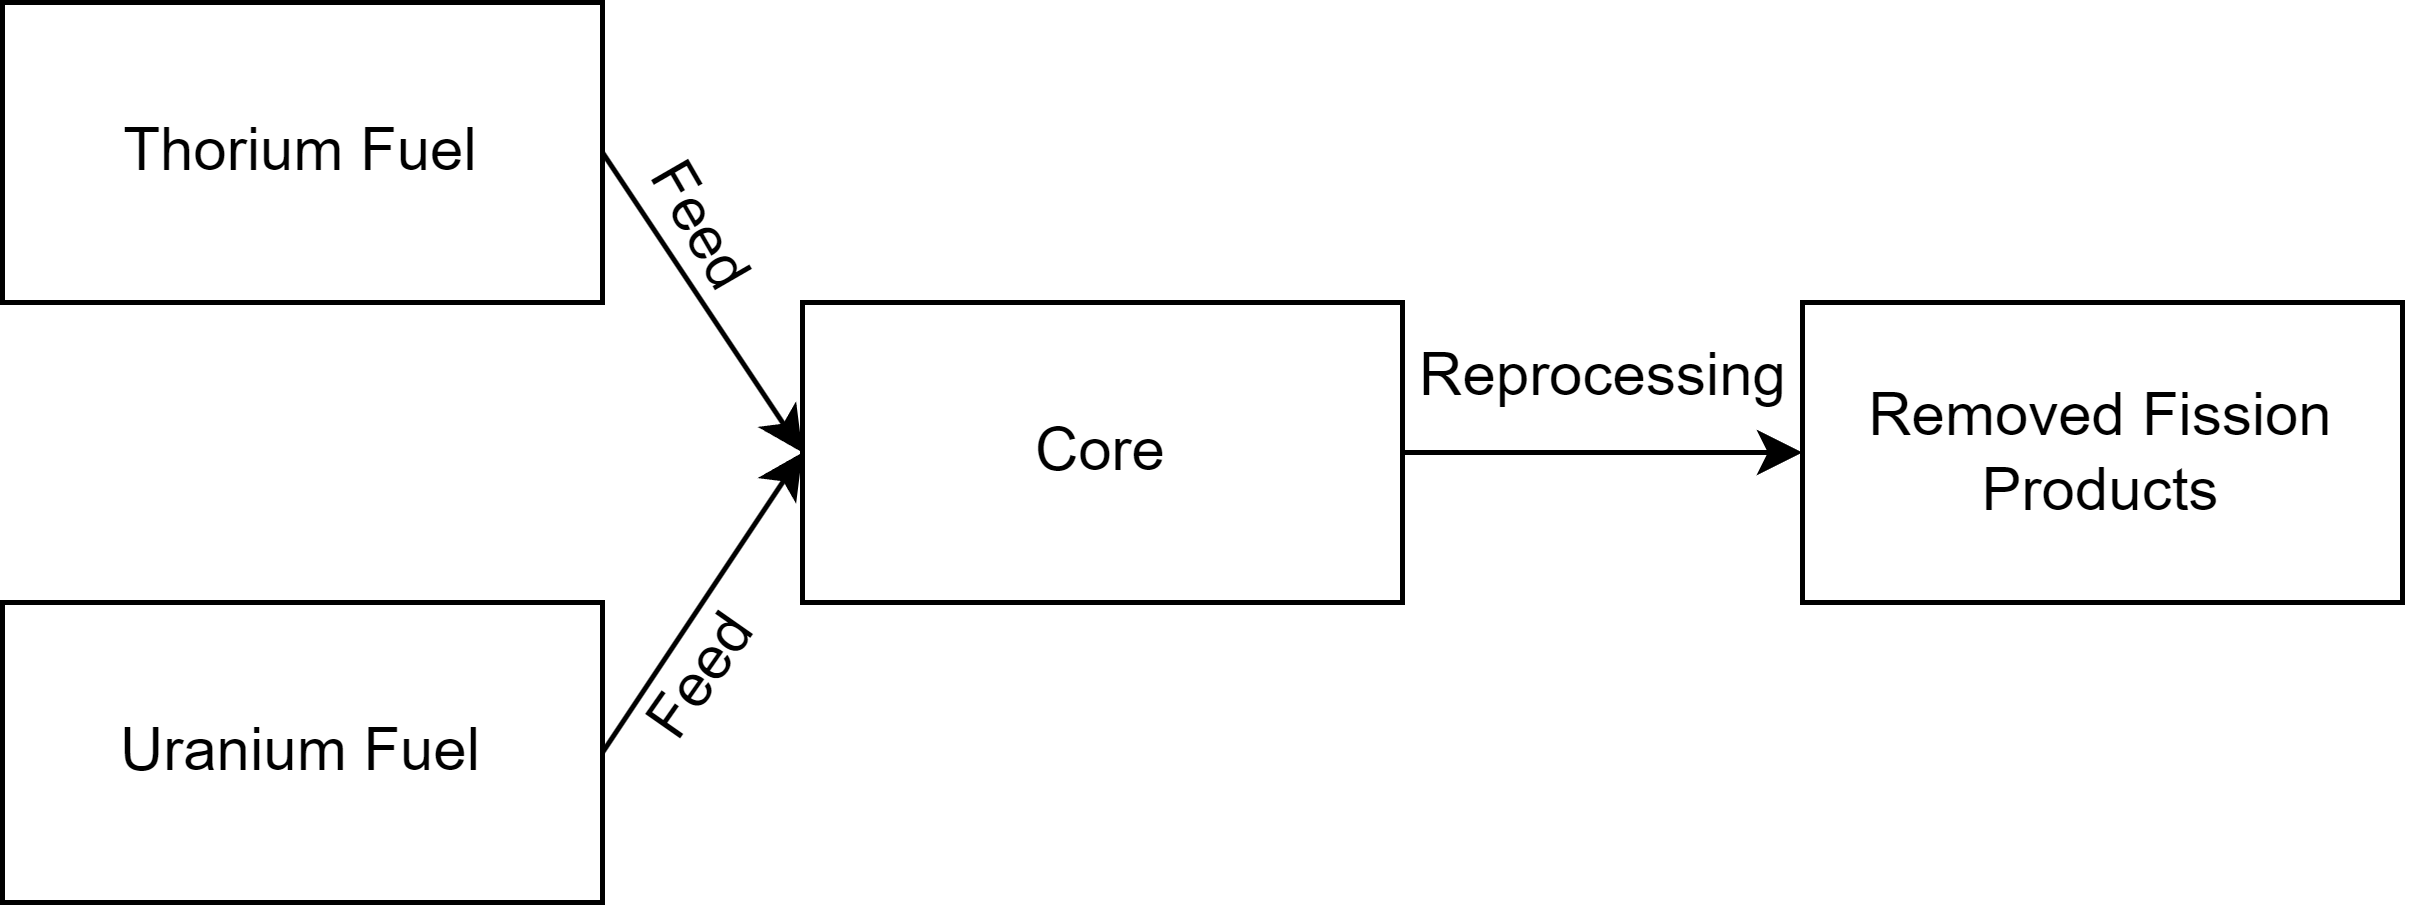
\includegraphics[scale=0.45]{images/sp-match-repr-scheme.png}
  \caption{Simplified reprocessing scheme based on mimicking SaltProc.}
   \label{fig:spmatchrepr}
\end{figure}

The second reprocessing scheme is physically based, and instead creates a protactinium decay tank. From this tank, any generated uranium is continuously removed and sent back to the core, which is the intended design scheme for the MSBR \cite{robertson_conceptual_1971}. A simplified version of the phyiscally realistic uranium feed can be seen in Figure \ref{fig:spmatchrepr}.

\begin{figure}[H]
  \centering
  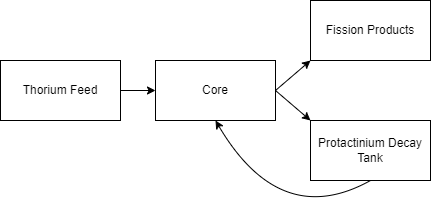
\includegraphics[scale=0.45]{images/phys-repr-scheme.png}
  \caption{Simplified reprocessing scheme based on the phyiscal MSBR processes.}
   \label{fig:spmatchrepr}
\end{figure}

Overall, it can be anticipated that the two methods will be approximately equal at steady-state, since at that point the assumption by Rykhlevskii that the uranium input is the same as the protactinium output should be valid. However, there is expected to be a fairly large difference for the first month or two of operation, as the half life of protactinium-233 is on the order of one month. This means that the uranium feed will take some time before it is providing a steady source of fissile material to the core.

